% !TEX root = ../thesis-example.tex
%
\chapter{Synchronisation}
\label{sec:Synchronisation}

\cleanchapterquote{The most important property of a program is whether it accomplishes the intention of its user.}{C.A.R. Hoare}{(British computer scientist,\\ winner of the 1980 Turing Award)}

Synchronisation beschreibt den Datenaustausch zwischen einem Sender und einem Empfänger. Dabei werden die Daten in Blöcke aufgeteilt und in einen Übertragungsrahmen eingepasst. Um die Daten aneinander anzugleichen muss festgestellt werden, welches Endgerät welche Daten besitzt und muss kontrolliert werden ob das andere Gerät eine Anforderung für diese Daten besitzt.

Besitzen beide Endgeräte dieselben Daten z.B. in unterschiedlichen Versionen, muss definiert werden, wie mit den Änderungen umgegangen werden soll.\cite[]{WEB:SYNCML:2014}

Aufgrund der Begrenzung des lokalen Gerätespeichers empfiehlt sich die Synchronisation auf zwei seperaten Wegen durchzuführen. Als Erstes wird die Datenbank synchronisiert und als Zweites alle Anhänge, wie z.B. Bilder oder Dokumente. So kann das Problem der Speicherbegrenzung bei Web Apps umgangen werden.

\section{Datenbanksynchronisation am Beispiel ``WebSqlSync''}
\label{sec:dbsync}

WebSqlSync\footnote{http://www.verious.com/code/orbitaloop/WebSqlSync/} ist eine Javascript Bibliothek zur automatischen Synchronisation einer lokalen WebSql Datenbank mit dem Server. Die Synchronisation erfolgt dabei in beide Richtungen und arbeitet auf dem Prinzip der inkrementellen Synchronisation, was bedeutet, dass nur erforderliche Daten übertragen werden.

WebSqlSync funktioniert auch ohne Internetverbindung. Alle Änderungen der Daten werden dabei verfolgt und mit dem Server abgeglichen, sobald wieder eine Internetverbindung besteht. Es wird auch die Änderung der Daten auf mehreren Geräten unterstützt.

Die Unterstützung von Webapp und der Phonegap App\footnote{http://phonegap.com/} für mobile Betriebssysteme wie z.B. iOS und Android ermöglicht eine einfache Integration ohne den Programmcode anpassen zu müssen.\cite[]{WEB:WEBSQLSYNC:2014}

\textbf{Installation und Initialisierung}

Um WebSqlSync nutzen zu können, muss nur die Datei webSqlSync.js im Head-Bereich im \ac{HTML} des Projekts hinzugefügt werden.

\lstset{language=html}
\lstinline$<script src="lib/webSqlSync.js" type="application/x-javascript" charset="utf-8"></script>$

Bei Aufruf der Bibliothek, werden automatisch zwei Datenbanktabellen erstellt, falls diese nicht bereits durch einen vorherigen Aufruf existieren. Die erste Tabelle \textbf{\lstinline$new_elem$} speichert alle neuen bzw. geänderten Elemente, die zweite Tabelle \textbf{\lstinline$sync_info$} das Datum der letzten Synchronisation.

Zusätzlich werden sogenannte SQLite Auslöser erstellt, die überwachen, ob Änderungen per \textbf{\lstinline$INSERT$} oder \textbf{\lstinline$UPDATE$} an den Tabellen vorgenommen wurden. SQLite ist eine einfache Datenbankbibliothek, die Befehle der Sprache \ac{SQL} verwendet.

Geänderte Elemente werden somit automatisch in der Tabelle \textbf{\lstinline$new_elem$} eingefügt.(Abb.\ref{code:initsync})

\begin{figure}[htb]
	\lstset{language=html}
	\begin{lstlisting}
	DBSYNC.initSync(
		TABLES_TO_SYNC, webSqlDb, sync_info,
		'http://www.myserver.com', callBackEndInit
	);\end{lstlisting}
	\caption{Codebeispiel für den Aufruf zur Datenbanksynchronisation}
	\label{code:initsync}
\end{figure}

\hspace{1 cm}

Die Tabellen die, mit dem Server synchronisiert werden sollen, werden in der Funktion \textbf{\lstinline$TABLES_TO_SYNC$} angegeben. (Abb.\ref{code:tabletosync})

\begin{figure}[htb]
	\lstset{language=html}
	\begin{lstlisting}
	TABLES_TO_SYNC = [
	  {tableName : 'table1', idName : 'the_id'},
	  {tableName : 'table2'}
	  //if idName not specified, it will assume that it's "id"
	];
	\end{lstlisting}
	\caption{Codebeispiel für die Datenbanktabellen die synchronisiert werden sollen}
	\label{code:tabletosync}
\end{figure}

\hspace{1 cm}

In der Tabelle \textbf{\lstinline$sync_info$} können alle Informationen gespeichert werden, die der Entwickler als nützlich empfindet, beispielsweise die Identifikation des Clients, da Sie mit an den Server gesendet wird. Dafür kann jegliche Information genutzt werden, wie z.B. die Emailadresse, ein Login oder auch eine entsprechende \ac{ID} des genutzten mobilen Endgeräts.

\textbf{Aufruf}

Um die Synchronisation zu starten wird die Funktion \textbf{\lstinline$syncNow$} aufgerufen. Die Synchronisation erfolgt dabei nach einer freiwählbaren Zeitspanne oder aber nach einer festgelegten Anzahl von Datenänderungen. (Abb.\ref{code:syncnow})

\begin{figure}[htb]
	\lstset{language=html}
	\begin{lstlisting}
	DBSYNC.syncNow(callBackSyncProgress, function(result) {
	  if (result.syncOK === true) {
	    //Synchronized successfully
	  }
	});
	\end{lstlisting}
	\caption{Codebeispiel für den Aufruf zur Synchronisation}
	\label{code:syncnow}
\end{figure}

\hspace{1 cm}

Bei größeren Datenmengen ist es für den Nutzer hilfreich, wenn dieser eine Fortschrittsanzeige erhält. Während der Synchronisation wird dafür bei jedem Einzelschritt, beispielsweise einzelne Datenpakete, die Funktion \textbf{\lstinline$callBackSyncProgress$} aufgerufen. (Abb.\ref{code:syncprocess})

\begin{figure}[htb]
	\lstset{language=html}
	\begin{lstlisting}
	callBackSyncProgress: function(message, percent, msgKey) {
	  $('#uiProgress').html(message+' ('+percent+'%)');
	},
	\end{lstlisting}
	\caption{Codebeispiel für den Callback zur Erstellung einer Fortschrittsanzeige}
	\label{code:syncprocess}
\end{figure}

\hspace{1 cm}

\textbf{Einschränkungen}

Die Bibliothek WebSqlSync besitzt auch ein paar wenige Einschränkungen. Zum Beispiel wird der \ac{SQL}-Befehl \textbf{\lstinline$DELETE$} nicht unterstützt. Stattdessen sollte dies mit einem update an der entsprechenden Stelle umgangen werden.

\section{Dateisynchronisation am Beispiel ``ownCloud''}
\label{sec:datasync}

ownCloud\footnote{https://owncloud.com/} ist eine Open Source Software zur Einrichtung einer unabhängigen serverseitigen Datenspeicherlösung. Sogenannte Cloudspeicher gibt es mittlerweile sehr viele. Die wohl bekanntesten sind Dropbox, Google Drive und OneDrive. Sie ermöglichen einen einfachen Datenzugriff von überall auf der Welt. Dafür lädt man seine Dateien über eine Internetverbindung auf einen speziellen Datenserver. Leider besitzt dies den großen Nachteil, dass mkeine 100 prozentige Sicherheit besteht, was mit den eigenen Daten passiert.

Um dies sicherzustellen bietet ownCloud die Möglichkeit einen eigenen Cloudserver\ref{Architektur} zu erstellen, auf dem der Nutzer alles selbst konfigurieren kann. Per Nutzer- und Rechteverwaltung lässt sich wie auf einem normalen Server festlegen, welcher Nutzer Dateien verändern kann.

Für die Daten werden Backup Lösungen angeboten, so dass jederzeit Sicherungen der Dateien angelegt werden können. Der wohl wichtigste Punkt ist jedoch die Verschlüsselung der gespeicherten Daten mittels \ac{SSL}. Dadurch können auch unternehmensrelevante Daten sicher gespeichert werden.

Durch die Open Source Lösung ownCloud lässt sich zu den bereits vorhandenen Plugins neue Software entwickeln und den eigenen Bedürfnissen anpassen. Da bereits Apps für die mobilen Betriebssystem (Abb.\ref{ownCloudApp}) zu Verfügung stehen, lassen sich relativ einfach Daten zwischen dem Server und dem Client synchronisieren.

Neben der frei verfügbaren ``Community Edition'' stehen für die volle Unterstützung der ownCloud Entwickler, welche bei Fragen zur Software oder den Apps zur Verfügung stehen, auch eine ``Business'' und eine ``Enterprise Version'' zur Verfügung, welche gegen eine jährliche Gebühr angeboten wird.\cite[]{WEB:OWNCLOUD:2014}

\hspace{2 cm}

\begin{figure}[htb]
	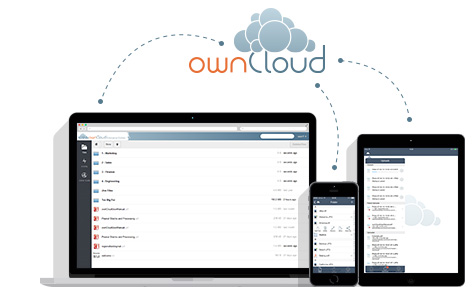
\includegraphics[width=\textwidth]{Bilder/architecture}
	\caption{Architektur ownCloud}
	\label{Architektur}
\end{figure}

\hspace{2 cm}

\textbf{Vorteile der Android/iOS App von ownCloud}

Die nachfolgenden Vor- und Nachteile der ownCloud App sind auf der Website https://owncloud.com/ beschrieben.\cite[]{WEB:OWNCLOUD:2014}

\begin{itemize}

	\item SSL- und HTTP-Verbindungen werden automatisch erkannt, so dass eine einfache und gesicherte Verbindung zu dem Server möglich wird.

	\item Dateien und Ordner auf dem Server können neu angelegt, durchsucht, umbenannt und gelöscht werden, je nachdem wie die Rechte an den Nutzer vergeben sind.

	\item Durch das Anlegen von Favoriten lassen sich Daten wie Dokumente, Bilder und Videos automatisch mit dem Server synchronisieren.

	\item Dateien können auf das mobile Endgerät heruntergeladen werden, um diese Offline nutzen zu können.

	\item Es werden durch die App mehrere ownCloud Accounts mit einem Device und zusätzlich die Anbindung an mehrere ownCloud Server unterstützt.

\end{itemize}

\hspace{2 cm}

\begin{figure}[htb]
	\begin{tabular}{l r}
		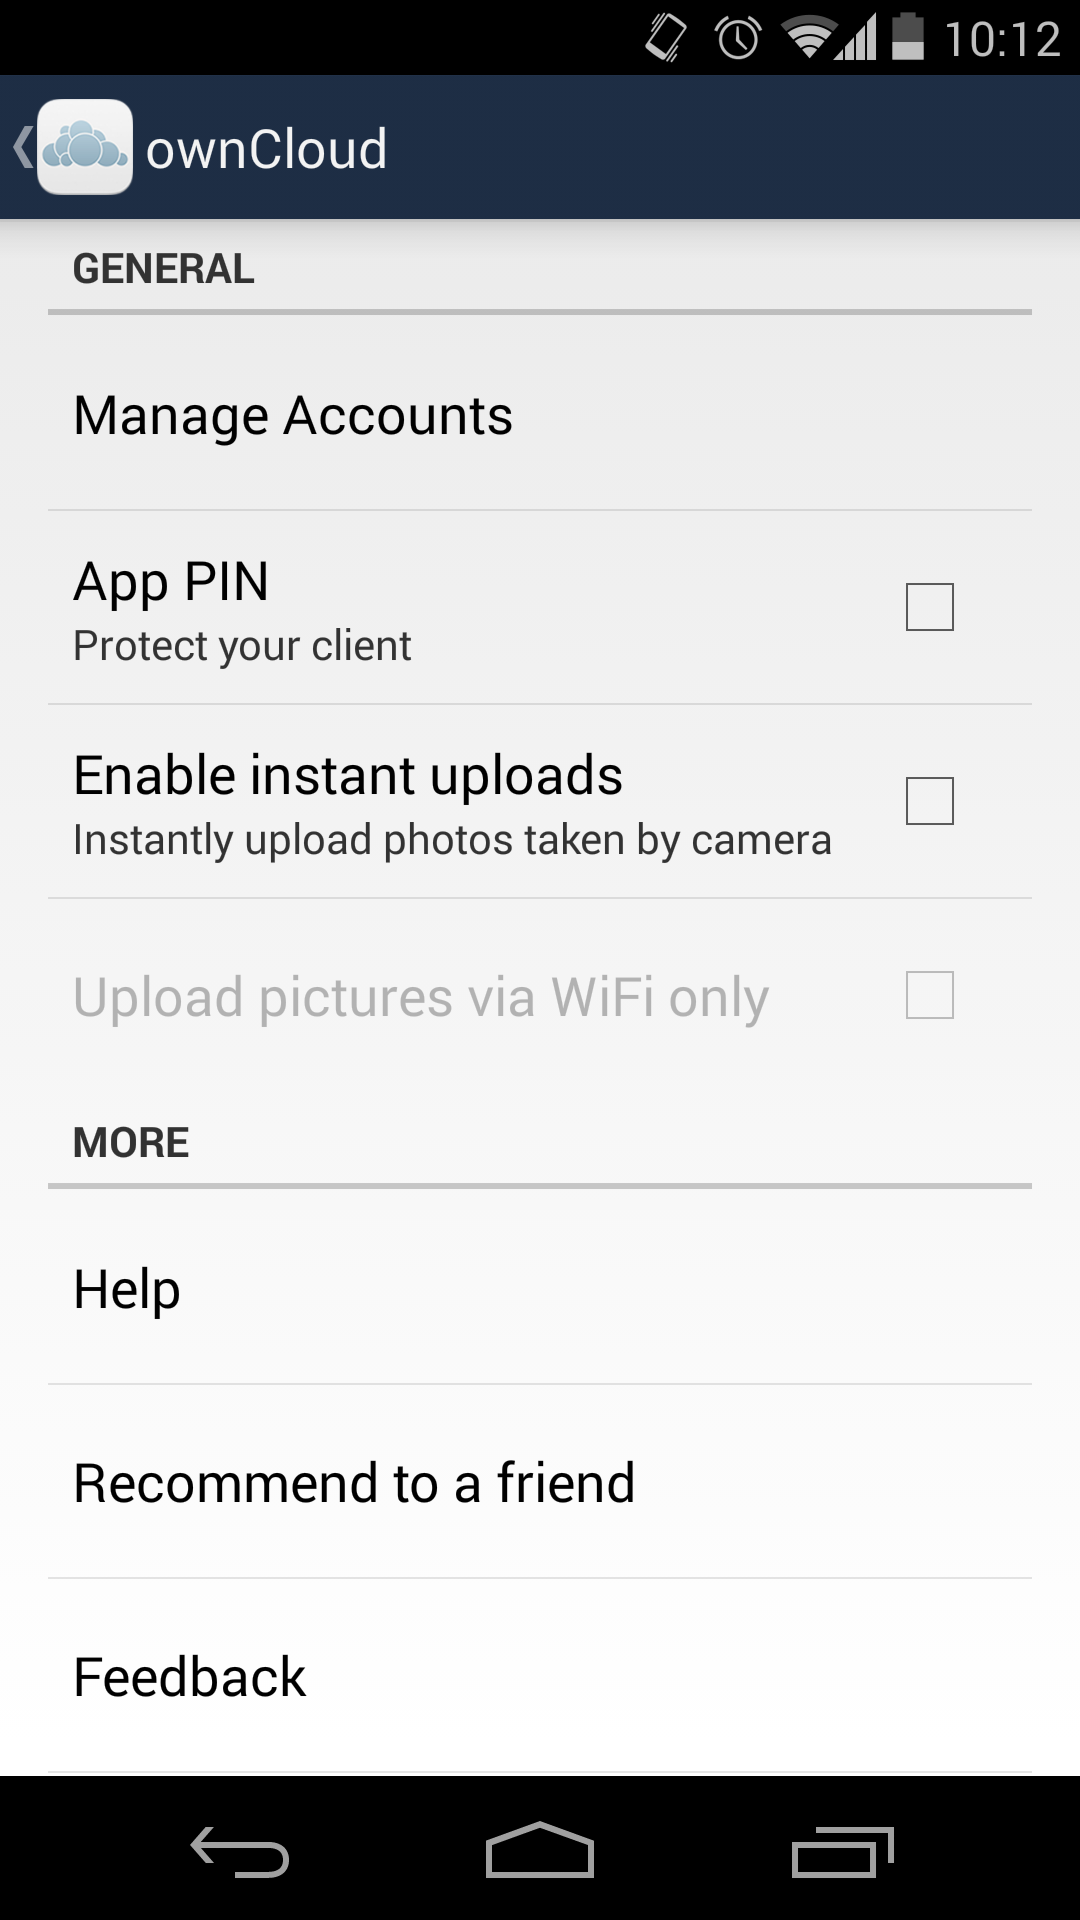
\includegraphics[width=0.49\textwidth]{Bilder/ownCloud-mobile1}
		&
		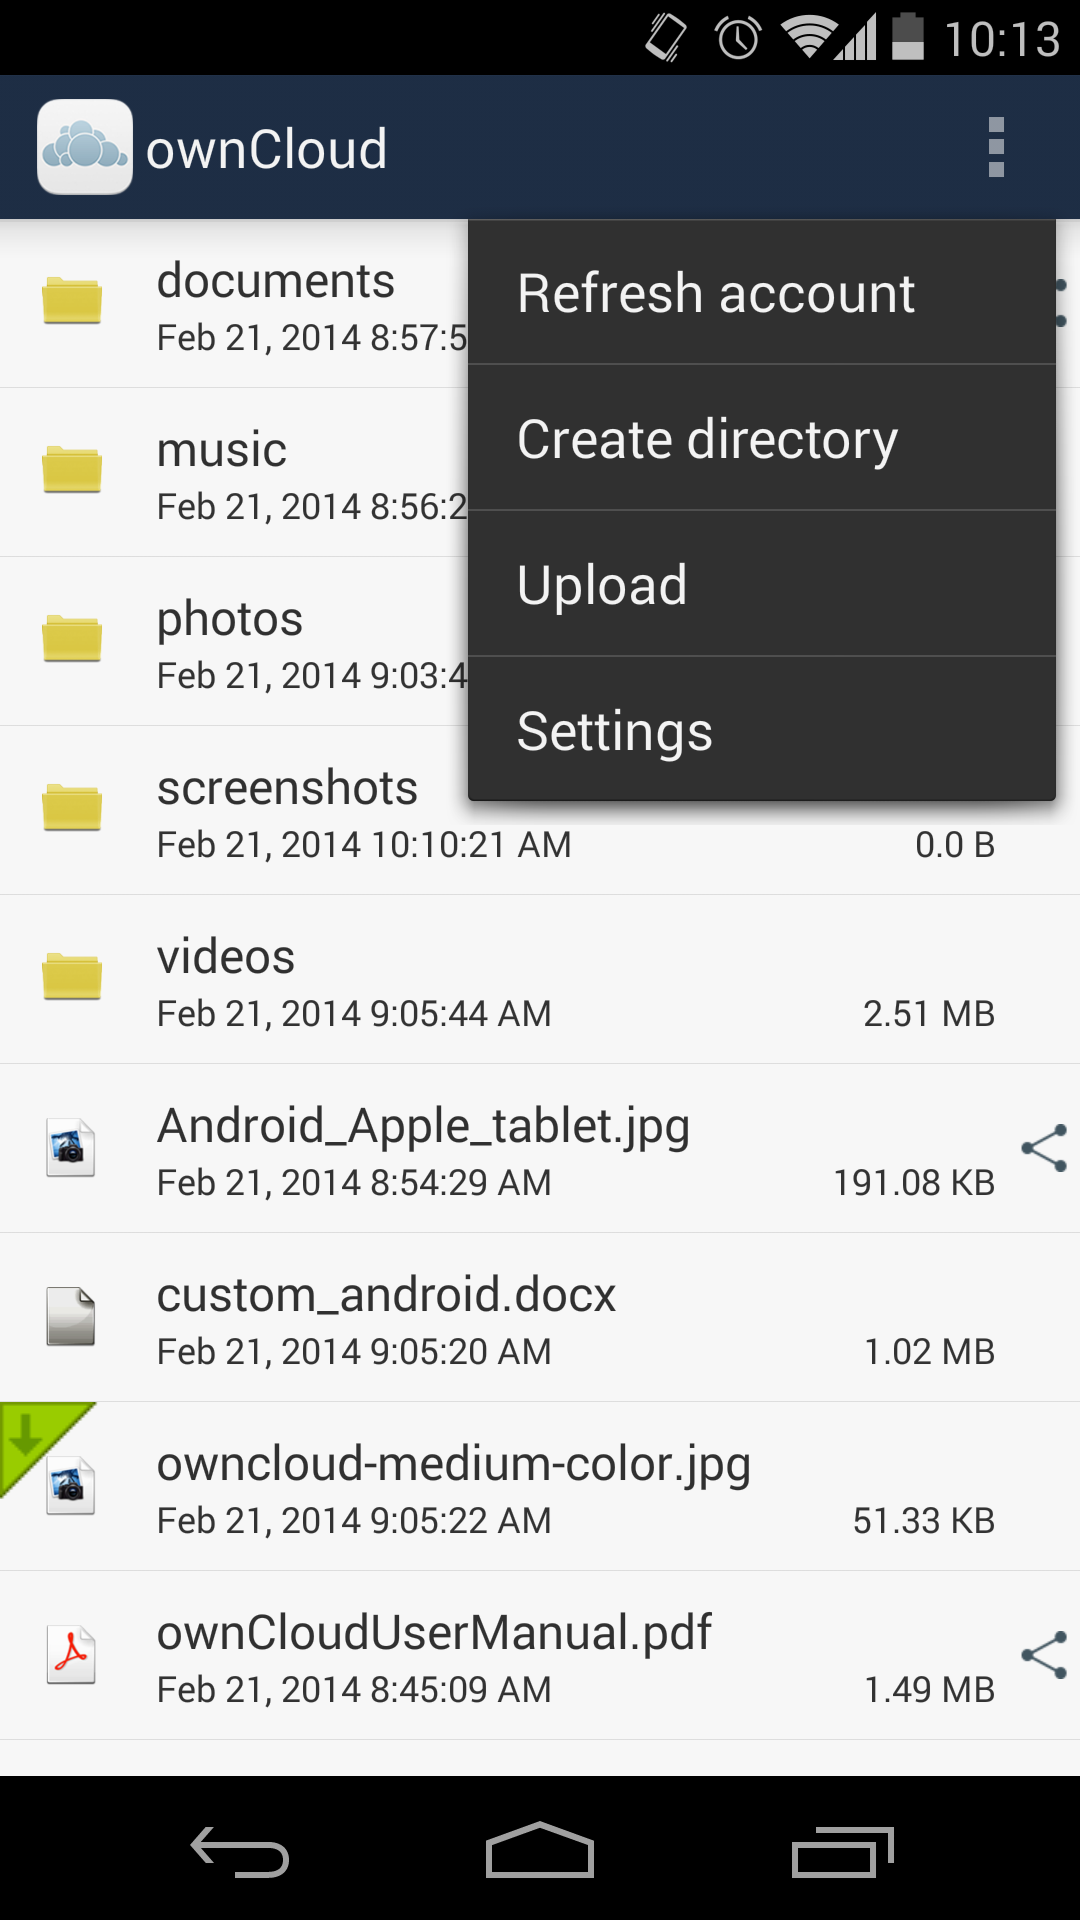
\includegraphics[width=0.49\textwidth]{Bilder/ownCloud-mobile2}
	\end{tabular}
	\caption{ownCloud App}
	\label{ownCloudApp}
\end{figure}

\hspace{2 cm}

Unabhängig von der Anzahl der Nutzer lassen sich mit dieser Cloudlösung auch die für die Datenbank aufgenommenen Bilder unkompliziert speichern. Egal ob ein Internetzugang zur Verfügung steht oder man Fotos offline aufgenommen und in einem Ordner von ownCloud ablegt werden, synchronisiert ownCloud diese automatisch sobald eine Internetverbindung zur Verfügung steht.

Einziger Nachteil ist dabei der hohe Kostenfaktor für die ``Enterprise'' Lösung, den man mit dem Kunden abstimmen muss. In Ausblick auf die Erweiterbarkeit durch die Open Source \ac{API} lässt sich die Software beliebig erweitern und kann somit den Nutzen-Kosten-Faktor verringern.
